% =====================================================================
% Introducao as Redes Neurais Artificiais
% Projeto 4 - Redes Neurais Recorrentes (LSTM e GRU)
% Autor: Henrique Crepaldi - RA 120410
%
% Observacao: eu escrevo este relatorio em primeira pessoa. Compilo o PDF
% no Overleaf. As figuras citadas estao na pasta "figuras_projeto4/".
% =====================================================================
\documentclass[11pt,a4paper]{article}

\usepackage[utf8]{inputenc}
\usepackage[T1]{fontenc}
\usepackage[brazil]{babel}
\usepackage[margin=2.5cm]{geometry}
\usepackage{graphicx}
\usepackage{amsmath}
\usepackage{booktabs}
\usepackage{float}
\usepackage{xcolor}
\usepackage[colorlinks=true,linkcolor=blue,urlcolor=blue]{hyperref}

\title{\textbf{Projeto 4 --- Redes Neurais Recorrentes (LSTM e GRU)}\\[4pt]
\large Previsão $t+k$ de uma série temporal de glicemia}
\author{Henrique Crepaldi --- RA 120410\\
Introdução às Redes Neurais Artificiais}
\date{\today}

\begin{document}
\maketitle

\begin{abstract}
Neste projeto eu implementei e comparei dois tipos de redes neurais
recorrentes --- \textbf{LSTM} e \textbf{GRU} --- para a tarefa de
\textbf{previsão $t+k$} em uma série temporal de glicemia. Dado um histórico
de 24 leituras (2 horas de dados, a cada 5 minutos), eu treinei os modelos
para prever o valor da glicose 30 minutos à frente ($k=6$ passos). Por se
tratar de um dado de saúde, eu optei por \emph{não} usar os dados reais da
minha bomba de insulina e gerei uma série sintética fisiologicamente
plausível, evitando qualquer questão de privacidade. Ajustei os
hiperparâmetros de cada arquitetura usando um conjunto de validação, analisei
as curvas de aprendizagem e avaliei o desempenho final em um conjunto de teste
nunca visto. Os dois modelos superaram com folga um \emph{baseline} ingênuo de
persistência; o GRU obteve o melhor resultado no teste
(RMSE $= 8{,}42$ mg/dL, $R^2 = 0{,}759$), e ainda com menos parâmetros que o
LSTM.
\end{abstract}

\section{Introdução e definição do problema}

A motivação deste projeto é pessoal: eu convivo com o monitoramento contínuo
de glicose (CGM), e antecipar para onde a glicemia está indo é clinicamente
muito útil para prevenir episódios de hipo e hiperglicemia. Formalmente, eu
tratei o problema como \textbf{previsão $t+k$}: a partir de uma janela de
leituras passadas, o modelo prevê o valor da glicose $k$ passos no futuro.

Escolhi redes recorrentes porque elas são naturalmente adequadas a sequências:
a cada passo de tempo elas atualizam um estado interno que resume o histórico
relevante. Comparei as duas arquiteturas recorrentes mais usadas, a LSTM
(\emph{Long Short-Term Memory}) e a GRU (\emph{Gated Recurrent Unit}), para
observar se a maior complexidade da LSTM traz vantagem neste problema.

\subsection{Sobre os dados: por que eu usei dados sintéticos}

Eu tenho acesso aos relatórios reais da minha bomba de insulina, mas decidi
\textbf{não utilizá-los} para evitar expor dados pessoais de saúde. No lugar,
eu gerei uma série sintética de glicemia que reproduz os principais fenômenos
fisiológicos. Essa é uma prática reconhecida em aprendizado de máquina aplicado
à saúde (existem simuladores consagrados, como o UVA/Padova). A minha série
contempla:

\begin{itemize}
  \item um \textbf{nível basal} de glicose (${\approx}100$ mg/dL em jejum);
  \item um \textbf{ritmo circadiano} suave ao longo das 24 horas;
  \item \textbf{picos pós-refeição} (café, almoço e jantar), com horário e
        intensidade variáveis a cada dia, modelados por uma curva que sobe e
        decai;
  \item o \textbf{efeito da insulina}, que puxa a glicose para baixo com um
        pequeno atraso após cada refeição;
  \item \textbf{ruído de sensor}, simulando a variabilidade da medição.
\end{itemize}

Eu gerei 60 dias de dados a cada 5 minutos, totalizando $17\,280$ leituras.
A Figura~\ref{fig:serie} mostra os três primeiros dias, com a faixa-alvo
clínica (70--180 mg/dL) destacada.

\begin{figure}[H]
  \centering
  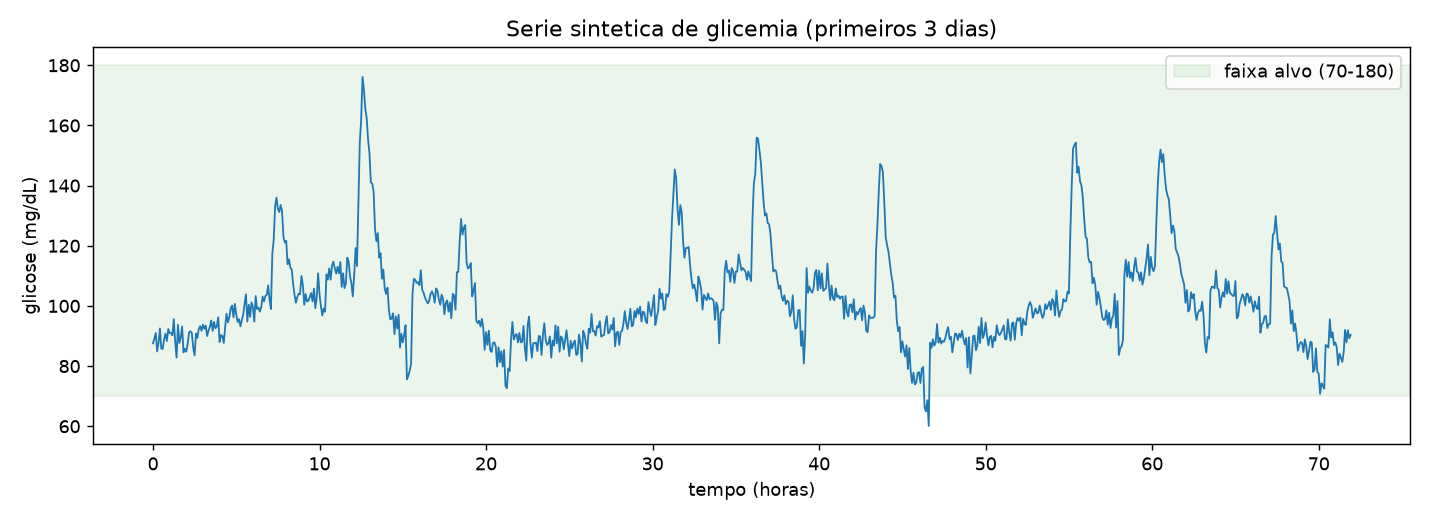
\includegraphics[width=0.95\textwidth]{figuras_projeto4/01_serie_glicemia.png}
  \caption{Trecho (3 dias) da série sintética de glicemia que eu gerei.
  Dá para ver os picos pós-refeição e o retorno gradual ao nível basal.}
  \label{fig:serie}
\end{figure}

\section{Metodologia}

\subsection{Janelamento para previsão $t+k$}

Eu transformei a série 1D em pares (entrada, alvo). Para cada instante $t$, a
entrada é a janela das $W$ leituras anteriores (inclusive $t$) e o alvo é a
leitura em $t+k$:
\begin{equation}
  \mathbf{x}_t = (g_{t-W+1}, \dots, g_{t}), \qquad y_t = g_{t+k}.
\end{equation}
Eu usei $W = 24$ (2 horas de histórico) e $k = 6$ (30 minutos à frente). Isso
gerou $17\,251$ janelas.

\subsection{Divisão temporal e cuidado com vazamento de dados}

Em séries temporais eu \textbf{não posso embaralhar os dados antes de dividir},
pois isso faria o modelo ``ver o futuro'' durante o treino --- um vazamento de
dados clássico. Por isso eu cortei a série em blocos contíguos, respeitando a
ordem do tempo: 70\% para treino (passado), 15\% para validação (meio) e 15\%
para teste (futuro), resultando em $12\,075$ / $2\,588$ / $2\,588$ amostras.

Pelo mesmo motivo, eu ajustei o normalizador (\emph{StandardScaler})
\textbf{apenas no conjunto de treino} e apenas apliquei a transformação em
validação e teste. Assim eu nunca uso estatísticas do futuro para normalizar o
passado. (Observo que, uma vez feita a divisão temporal em blocos, cada janela
já é um exemplo independente; por isso eu posso embaralhar as janelas
\emph{dentro} do treino com segurança, o que ajuda o gradiente, mantendo
validação e teste em ordem para os gráficos.)

\subsection{Arquitetura dos modelos}

Eu defini uma única arquitetura parametrizável, trocando apenas o tipo de
célula recorrente (LSTM ou GRU) para que a comparação fosse justa:
\begin{enumerate}
  \item uma camada recorrente (LSTM ou GRU), possivelmente empilhada, que
        processa a janela e produz um estado oculto a cada passo;
  \item eu tomo o estado oculto do \textbf{último passo} como resumo da janela;
  \item uma camada densa linear projeta esse estado em um único valor: a
        glicose prevista em $t+k$ (é uma regressão, então a saída é linear).
\end{enumerate}
Usei \emph{dropout} de $0{,}2$ entre camadas (quando há mais de uma) como
regularização, função de perda MSE e otimizador Adam.

\subsection{Ajuste de hiperparâmetros com o conjunto de validação}

Eu realizei uma busca em grade, separadamente para LSTM e GRU, variando:
\begin{itemize}
  \item tamanho do estado oculto: $\{32,\ 64\}$;
  \item número de camadas recorrentes: $\{1,\ 2\}$;
  \item taxa de aprendizado: $\{10^{-2},\ 10^{-3}\}$.
\end{itemize}
Para cada uma das 8 configurações eu treinei o modelo e usei a
\textbf{menor perda de validação} como critério de seleção. A
Tabela~\ref{tab:busca} resume os melhores achados.

\begin{table}[H]
  \centering
  \caption{Melhor configuração encontrada para cada arquitetura, segundo a
  perda (MSE, normalizada) no conjunto de validação.}
  \label{tab:busca}
  \begin{tabular}{lcccc}
    \toprule
    Modelo & Estado oculto & Camadas & Taxa aprend. & Val.\ MSE \\
    \midrule
    LSTM & 64 & 1 & $10^{-2}$ & 0{,}2323 \\
    GRU  & 32 & 1 & $10^{-2}$ & 0{,}2397 \\
    \bottomrule
  \end{tabular}
\end{table}

\subsection{Critério de parada (early stopping)}

Para cada treino, eu monitorei a perda de validação e interrompi o treinamento
quando ela parava de melhorar por um número fixo de épocas (paciência),
restaurando os melhores pesos. Isso me protege contra o overfitting, que fica
bem visível nas curvas de aprendizagem.

\subsection{Reprodutibilidade}

Como eu faço em todos os projetos, fixei a semente \texttt{SEED = 42} em todas
as fontes de aleatoriedade (\texttt{random}, \texttt{numpy}, \texttt{torch}) e
re-semeei antes de cada treino, para que a comparação entre LSTM e GRU seja
justa e os resultados reproduzíveis.

\section{Resultados}

\subsection{Curvas de aprendizagem}

A Figura~\ref{fig:curvas} mostra as curvas de treino e validação dos dois
modelos. A perda de treino cai de forma consistente, enquanto a de validação
estabiliza e passa a subir a partir de aproximadamente a 12\textsuperscript{a}
época --- o sinal clássico de overfitting. Foi exatamente esse comportamento
que o meu critério de parada capturou: os pesos finais correspondem ao ponto de
menor perda de validação, antes da degradação.

\begin{figure}[H]
  \centering
  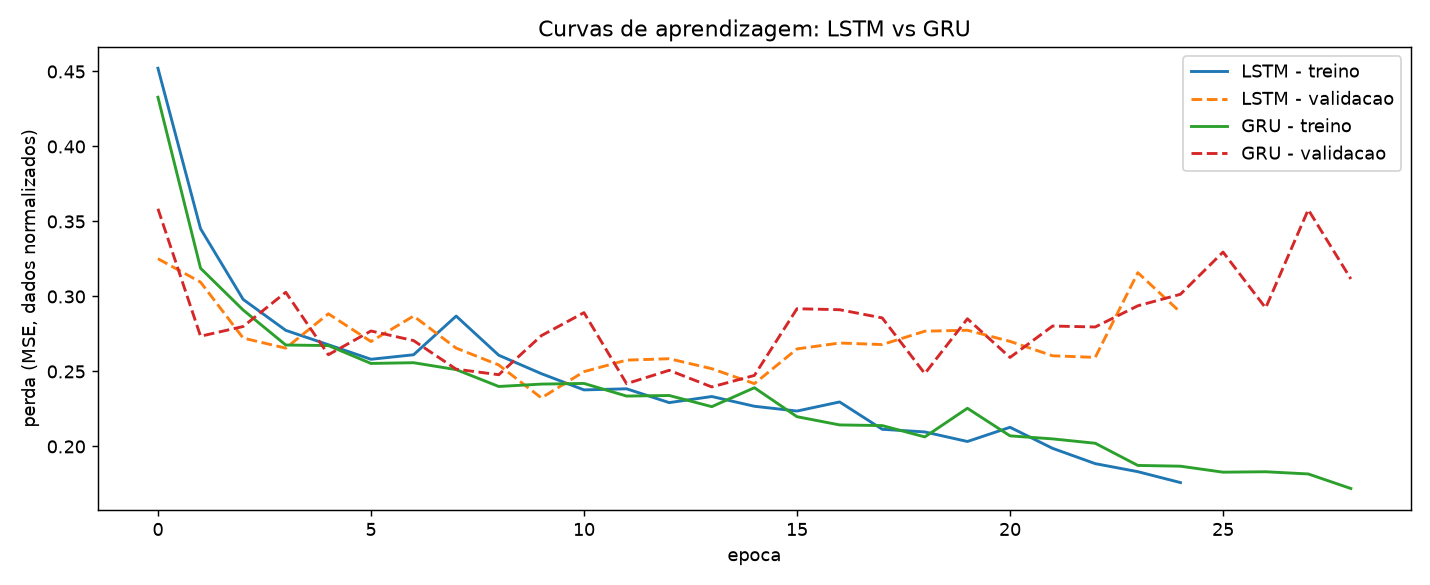
\includegraphics[width=0.95\textwidth]{figuras_projeto4/02_curvas_aprendizagem.png}
  \caption{Curvas de aprendizagem (treino e validação) para LSTM e GRU. A
  divergência entre treino e validação justifica o uso de early stopping.}
  \label{fig:curvas}
\end{figure}

\subsection{Qualidade da previsão}

A Figura~\ref{fig:prev} compara as previsões com o valor real em um trecho do
conjunto de teste. Os dois modelos acompanham bem a tendência geral e os picos
pós-refeição. Como é esperado para um horizonte de 30 minutos, eu noto que as
redes \textbf{suavizam e atrasam levemente os picos mais abruptos} --- prever
uma subida brusca com antecedência é genuinamente difícil, e esse é o tipo de
erro que mais aparece.

\begin{figure}[H]
  \centering
  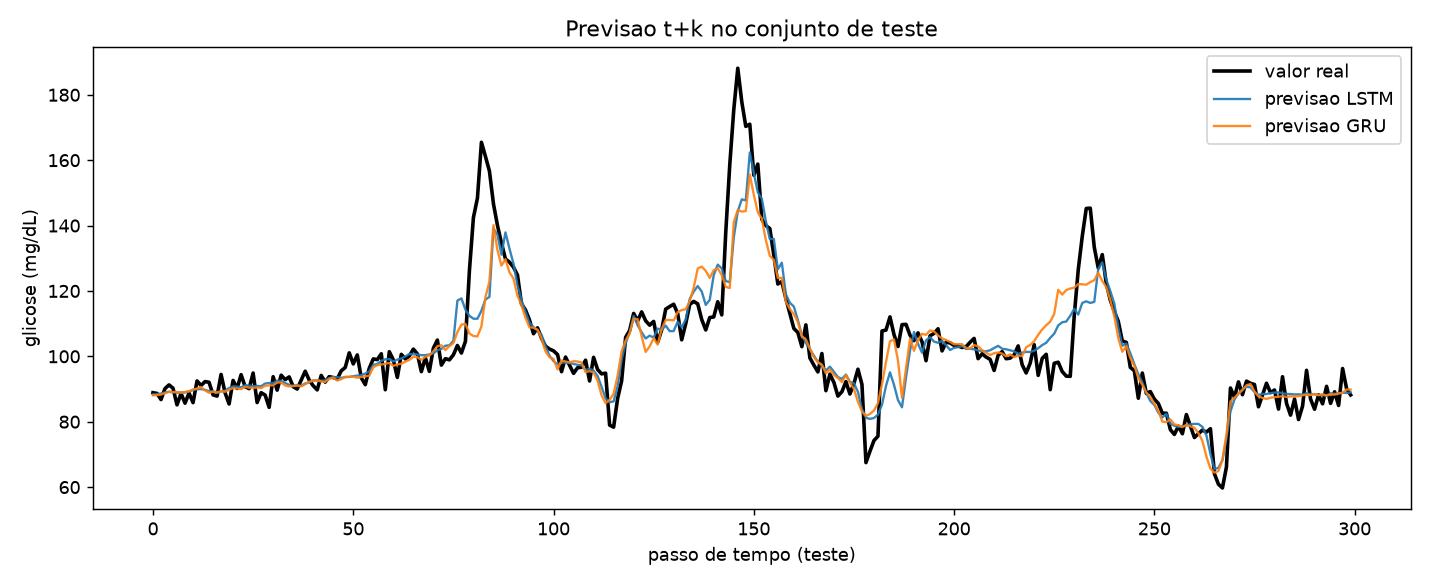
\includegraphics[width=0.95\textwidth]{figuras_projeto4/03_previsoes_teste.png}
  \caption{Previsão $t+k$ (30 min à frente) no conjunto de teste, comparada ao
  valor real.}
  \label{fig:prev}
\end{figure}

A Figura~\ref{fig:disp} mostra o gráfico de dispersão (previsto $\times$ real).
Os pontos se concentram em torno da reta ideal $y = x$, indicando pouco viés
sistemático em ambos os modelos.

\begin{figure}[H]
  \centering
  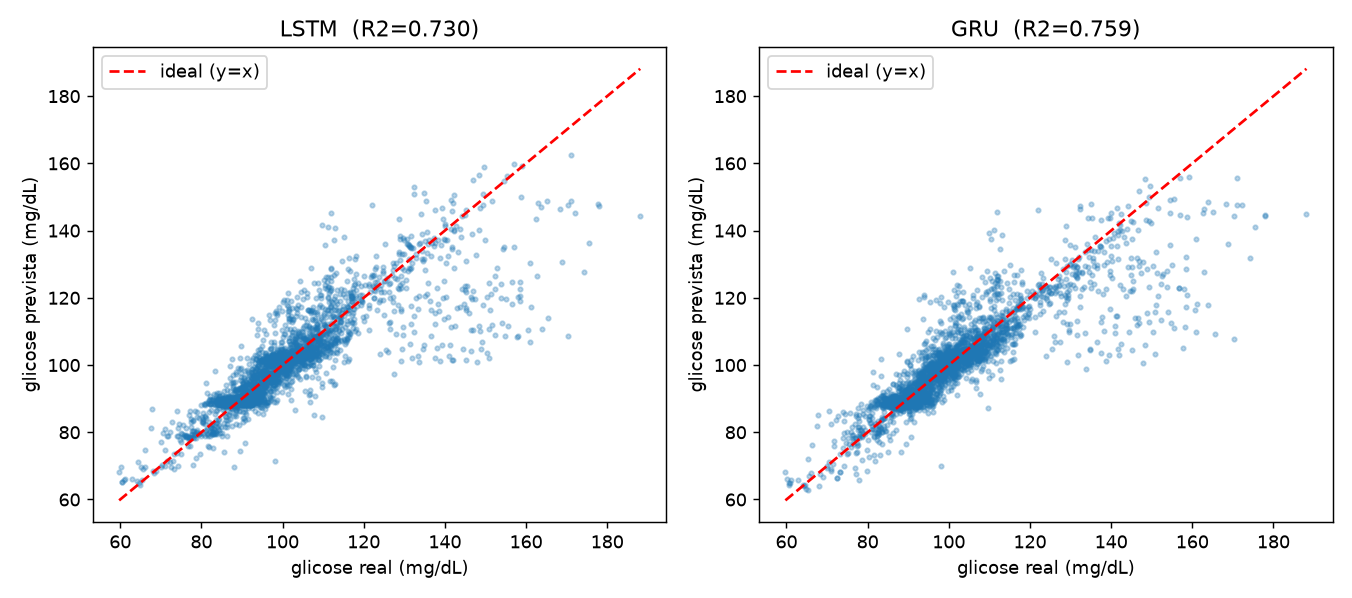
\includegraphics[width=0.95\textwidth]{figuras_projeto4/04_dispersao.png}
  \caption{Dispersão previsto $\times$ real no teste. Quanto mais próximo da
  reta tracejada ($y=x$), melhor.}
  \label{fig:disp}
\end{figure}

\subsection{Métricas de avaliação}

A Tabela~\ref{tab:metricas} reúne as métricas no conjunto de teste. Além de
RMSE, MAE e $R^2$, eu incluí uma métrica clínica: a fração de previsões
``aceitáveis'' segundo um critério 15/15 (erro dentro de 15 mg/dL para valores
baixos ou de 15\% para valores altos). Como referência, incluí também um
\textbf{baseline ingênuo} de persistência, que simplesmente prevê que a glicose
daqui a 30 minutos será igual à atual.

\begin{table}[H]
  \centering
  \caption{Desempenho no conjunto de teste. Menor é melhor para RMSE e MAE;
  maior é melhor para $R^2$ e para a métrica clínica.}
  \label{tab:metricas}
  \begin{tabular}{lcccc}
    \toprule
    Modelo & RMSE (mg/dL) & MAE (mg/dL) & $R^2$ & Aceitáveis 15/15 (\%) \\
    \midrule
    LSTM     & 8{,}90  & 5{,}21 & 0{,}730 & 94{,}4 \\
    \textbf{GRU} & \textbf{8{,}42} & \textbf{5{,}03} & \textbf{0{,}759} & \textbf{95{,}0} \\
    \midrule
    Baseline (persistência) & 14{,}81 & 9{,}72 & --- & --- \\
    \bottomrule
  \end{tabular}
\end{table}

\section{Discussão}

Alguns pontos que eu destaco a partir dos resultados:

\begin{itemize}
  \item \textbf{As redes aprenderam algo real.} Ambas superaram o baseline de
        persistência com folga (RMSE ${\approx}8{,}4$--$8{,}9$ contra
        $14{,}81$ mg/dL). Isso confirma que os modelos não estão apenas
        copiando o último valor observado.

  \item \textbf{O GRU venceu, e com menos parâmetros.} A melhor configuração do
        GRU usa estado oculto de 32 (contra 64 do LSTM) e ainda assim obteve o
        menor RMSE e o maior $R^2$ no teste. Para este problema, a maior
        complexidade do LSTM não se traduziu em vantagem --- um resultado
        coerente com a literatura, que mostra GRU e LSTM frequentemente
        empatados, com o GRU levando vantagem quando há menos dados ou quando
        se busca eficiência.

  \item \textbf{Overfitting controlado.} As curvas de aprendizagem deixam claro
        o momento em que a validação começa a piorar; o early stopping evitou
        que eu levasse esse sobreajuste para a avaliação final.

  \item \textbf{Limitação honesta.} O erro se concentra nos picos abruptos.
        Para um horizonte de 30 minutos isso é esperado, mas sugere caminhos de
        melhora: aumentar a janela de entrada, incluir variáveis exógenas
        (p.\,ex.\ carboidratos e doses de insulina como \emph{features}
        adicionais) ou prever a tendência (subindo/descendo) em paralelo ao
        valor.
\end{itemize}

\section{Conclusão}

Eu implementei um pipeline completo de previsão $t+k$ com redes recorrentes,
desde a geração de uma série de glicemia sintética e livre de dados pessoais
até a avaliação final em teste, passando pelo ajuste de hiperparâmetros em
validação e pela análise das curvas de aprendizagem. Os dois modelos previram a
glicemia 30 minutos à frente com erro médio em torno de 5 mg/dL e cerca de 95\%
de previsões clinicamente aceitáveis, superando claramente o baseline ingênuo.
O GRU apresentou o melhor compromisso entre precisão e simplicidade, sendo a
minha escolha final para este problema.

\section*{Reprodução}

Para reproduzir, basta executar \texttt{python rnn\_glicemia\_project4.py}. O
script gera a série, faz a busca de hiperparâmetros, treina os modelos finais,
avalia no teste e salva todas as figuras na pasta \texttt{figuras_projeto4/}.
Dependências: \texttt{torch}, \texttt{numpy}, \texttt{pandas},
\texttt{matplotlib} e \texttt{scikit-learn}.

\end{document}
